\documentclass{report}
\usepackage[utf8]{inputenc}
\usepackage{amsmath}
\usepackage{indentfirst}
\usepackage{graphicx}
\usepackage{subfigure}
\usepackage{float} 
\setlength{\parindent}{2em}
\usepackage{booktabs}
\usepackage{multirow}
\usepackage{geometry}
\usepackage{xeCJK}

\geometry{a4paper,scale=0.77}


\title{\textbf{ENGG1350 Experiment Report} \\ {\small Viscosity by a Falling Particle}}
\author{Entong He}
\date{October 2021}

\begin{document}

\maketitle
\section{Background Information}
This section introduces the principle of the experiment, and gives the derivation of the Stokes' Law.
\subsection{History}


\noindent George G. Stokes\footnote{Stokes, G. G. (1851). "On the effect of internal friction of fluids on the motion of pendulums". Transactions of the Cambridge Philosophical Society. 9, part ii: 8–106. } gave the analytical solution of the drag force applied on definite particle by arbitrary fluid
\begin{equation}
F = 6 \pi \mu R v ~\footnote{ $\mu$: viscous coefficient; R: radius of the sphere particle; v: flow velocity relative to the particle}
\end{equation}
This equation is tenable only under the circumstance that the fluid is of low Reynolds number, and no turbulence occurs. 
\subsection{Derivation}
\indent \par
The Navier-Stokes equation describe the behaviour of a certain fluid 
\begin{equation}
\ \rho [ \frac{\partial \vec v}{\partial t} + (\vec v \nabla) \vec v] = -\nabla \vec p + \mu \nabla^2 \vec v\
\end{equation}
In low-Reynolds assumption, the left hand side can be neglected, we have
\begin{equation}
\ \nabla \vec p = \mu \nabla^2 \vec v\
\end{equation}
Take curl in both side to eliminate the term of \(p\), since in polar
coordinate the velocity of fluid is easier to analyse. \par
\begin{equation}
\begin{aligned}
    \nabla \times (\nabla \times p) &= \mu[\nabla \times (\nabla^2 \vec v )] \\ &
    = \mu \nabla \times [\nabla (\nabla \vec v)  - \nabla \times (\nabla \times \vec v)] \\ & = -\mu \nabla \times [\nabla \times (\nabla \times \vec v)] \\ & = 0 \notag
\end{aligned}
\end {equation}
\par
\indent Equality above shows that
$ \nabla \times[\nabla \times (\nabla \times \vec v)] = 0 $.
~~ Let
\begin{equation}
    \nabla \times \vec v = \vec \zeta ~\footnote{Moffatt, H.K. (2015), "Fluid Dynamics", in Nicholas J. Higham; et al. (eds.), The Princeton Companion to Applied Mathematics, Princeton University Press, pp. 467–476} \notag  
\end{equation} 
\indent \par
\noindent Then we have
\begin{equation}
\begin{aligned}
    \nabla \times(\nabla \times \vec \zeta) &= \nabla^2 \vec \zeta - \nabla(\nabla
     \vec \zeta) \\ & = \nabla^2 \vec \zeta = 0.
\end{aligned}
\end{equation} 
\clearpage

\indent \par
\noindent
In 2-Dimensional coordinates, $\zeta_{z} = \frac{\partial u}{\partial y} - \frac{\partial v}{\partial x}$. We may well assume that 
\begin{equation}
u = -\frac{\partial \psi}{\partial y }, ~
v = \frac{\partial \psi}{\partial x},
\end{equation}
we then obtain
\begin{equation}
\begin{aligned}
    \zeta_{z} &= -\frac{\partial^2 \psi}{\partial y^2} - \frac{\partial^2 \psi}{\partial x^2} \\ & = -\nabla^2 \psi.
\end{aligned}
\end{equation}
\indent \par
\noindent
Now we are attempting to solve PDE
\begin{equation}
    \nabla^2(\nabla^2 \psi) = 0.
\end{equation}
\indent \par
We observe the fluid faraway from the sphere particle. Assume that it flows with a stable velocity $u_{\infty}$. Then $v_{r} = u_{\infty} cos\theta ,~ v_{\theta} = -u_{\infty} sin\theta$. We have
\begin{equation}
\begin{aligned}
    v_{r} &= \frac{1}{r^2 sin\theta} \frac{\partial \psi}{\partial \theta} = u_{\infty}cos\theta \\
    v_{\theta} &= -\frac{1}{r sin\theta} \frac{\partial \psi}{\partial r} = -u_{\infty}sin\theta.
\end{aligned}
\end{equation}
\indent \par
\noindent
From equation (8) we obtain
\begin{equation}
\begin{aligned}
    \psi &= \frac{u_{\infty} r^2}{2}sin^2\theta + f_{1}(r) \\
    & = \frac{u_{\infty} r^2 }{2} sin^2\theta + f_{2}(\theta).
\end{aligned}
\end{equation}
\indent The solution shows that $\psi$ can be written as 
\begin{equation}
    \psi = f(r)sin^2(\theta)
\end{equation}
If we write $f(\theta) = \sum_{i \in D} C_{i}r^{i}$, then every term in the summation serve the equation above.
Substitute $\psi =f(\theta)sin^2(\theta) = Cr^{n}sin^2\theta$ back to PDE (7), we obtain
\begin{equation}
\begin{aligned}
    \nabla^2\psi &= [\frac{\partial}{\partial r^2} + \frac{sin\theta}{r^2} \frac{\partial}{\partial \theta}(\frac{1}{sin\theta} \frac{\partial}{\partial \theta})]Cr^{n}sin^2\theta \\ 
    & = C[n(n-1) -2]sin^2\theta r^{n-2} \notag
\end{aligned}
\end{equation}
\begin{equation}
    \nabla^2(\nabla^2 \psi) = C[n(n-1)-2][(n-2)(n-3) -2]sin^2\theta r^{n-4} = 0.
\end{equation}
Then we conclude that
\begin{equation}
    n_1 = -1,~n_2 = 1,~ n_3 = 2,~n_4 = 4,
\end{equation}
that is,
\begin{equation}
    f(r) = \frac{C_1}{r} + C_2r + C_3r^2 + C_4r^4.
\end{equation}
\indent Boundary conditions indicate the feature of fluid in three cases: 
\textcircled{\small1}No penetration,~\textcircled{\small2}No slip,~\textcircled{\small3}No disturbance to fluid at infinity.~That is
\begin{equation}
\begin{aligned}
    &v_r \bigg|_{r = R} = \frac{1}{r^2sin\theta}\frac{\partial}{\partial \theta} f(r)sin^2\theta \bigg|_{r = R} = 0 \\ 
    &v_{\theta} \bigg|_{r = R} = -\frac{1}{rsin\theta}\frac{\partial}{\partial r}f(r)sin^2\theta \bigg|_{r = R} = 0 \\
    &v_r \bigg|_{r \rightarrow \infty} = u_{\infty}cos\theta
\end{aligned}
\end{equation}
\clearpage

Substituting equation (13) to (14), we obtain
\begin{equation}
    C_1 = \frac{u_{\infty}R^3}{4},~C_2 = -\frac{3}{4}u_{\infty}R,~C_3 = \frac{u_{\infty}}{2},~C_4 = 0.
\end{equation}
Then 
\begin{equation}
\begin{aligned}
    &\psi = \frac{u_{\infty}r^2}{2}sin^2\theta(1-\frac{3}{2}\frac{R}{r} + \frac{R^3}{2r^3}) \\
    &v_{r} = u_{\infty}cos\theta(1-\frac{3}{2}\frac{R}{r} + \frac{R^3}{2r^3}) \\
    &v_{\theta} = u_{\infty}sin\theta(\frac{R^3}{4r^3} + \frac{3}{4} \frac{R}{r} - 1)
\end{aligned}
\end{equation}
\indent Back to the original equation (3)
\begin{equation}
\begin{aligned}
    \nabla^2 \vec v &= [\frac{1}{r^2}\frac{\partial}{\partial r}(r^2 \frac{\partial}{\partial r}) + \frac{1}{r^2sin\theta}\frac{\partial}{\partial \theta} (sin\theta \frac{\partial}{\partial \theta} ) + \frac{1}{r^2 sin^2\theta} \frac{\partial^2}{\partial \phi^2}](v_r \hat e_r + v_{\theta} \hat e_{\theta}) \\
    & = \hat e_r (\frac{\partial^2 v_r}{\partial r^2} + \frac{1}{r^2} \frac{\partial^2 v_r}{\partial \theta^2} + \frac{2}{r} \frac{\partial v_r}{\partial r} + \frac{cot\theta}{r^2}\frac{\partial v_r}{\partial \theta} - \frac{2}{r^2}v_r -\frac{2cot\theta}{r^2}v_{\theta} -\frac{2}{r^2}\frac{\partial v_{\theta}}{\partial \theta}) \\ &+
    \hat e_{\theta}(\frac{\partial^2 v_{\theta}}{\partial r^2} + \frac{1}{r^2} \frac{\partial^2 v_{\theta}}{\partial \theta^2} + \frac{2}{r}\frac{\partial v_{\theta}}{\partial r} + \frac{cot\theta}{r^2} \frac{\partial v_{\theta}}{\partial \theta} - \frac{1}{r^2 sin^2 \theta}v_{\theta} + \frac{2}{r^2} \frac{\partial v_{\theta}}{\partial \theta}) \notag
\end{aligned}
\end{equation}
\noindent Then we obtain
\begin{equation}
\begin{aligned}
    &\frac{1}{\mu} \frac{\partial p}{\partial r} = \frac{3u_{\infty}cos\theta R}{r^3} \\ &\frac{1}{\mu} \frac{\partial p}{r \partial \theta} = \frac{3u_{\infty}sin\theta R}{2r^3}
\end{aligned}
\end{equation}
Solve the equations above, we obtain
\begin{equation}
\begin{aligned}
    p(r,\theta) &= -\frac{3u_{\infty}cos\theta \mu R }{2r^2} + f_1(\theta) \\
    & = -\frac{3u_{\infty}cos\theta \mu R}{2r^2} + f_2(r) 
\end{aligned}    
\end{equation}
We can simplify the equations by assuming $f_1(\theta) = f_2(r) = Const$. To find out the constant we can use boundary condition that
\begin{equation}
    \lim_{r \rightarrow \infty}p = p_{\infty}
\end{equation}
Then $Const = p_{\infty}$. Hence
\begin{equation}
    p(r,\theta) = -\frac{3u_{\infty}cos\theta \mu R }{2r^2} + p_{\infty}.
\end{equation}

\indent For the viscous stress
\begin{equation}
\begin{aligned}
    &\tau_{rr} = 2\mu \frac{\partial v_r}{\partial r} = 2u_{\infty} \mu cos\theta (\frac{3R}{2r^2} -\frac{3R^3}{2r^4}) \\
    &\tau_{r\theta} = \mu[r\frac{\partial}{\partial r}(\frac{v_{\theta}}{r}) + \frac{1}{r} \frac{\partial v_{r}}{\partial \theta}] = -\frac{3 u_{\infty} \mu sin\theta R^3}{2r^4}
\end{aligned}
\end{equation} 
\indent
\graphicspath{ {./ENGG1350 Experiment Data/} }
\centerline{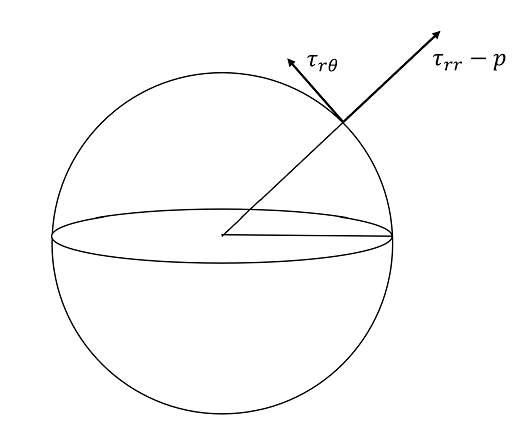
\includegraphics[height = 5.12cm]{Auxiliary Files/ENGG1350 Experiment Data/1350 image.png}}
\centerline{Figure 1.2.1 Diagram of Drag Force}

\clearpage

\noindent The contribution of every area element is
\begin{equation}
    dF = [\tau_{r\theta} \bigg|_{r = R} sin\theta - (\tau_{rr} \bigg|_{r = R} - p)cos\theta]~2\pi R^2sin\theta d\theta \notag
\end{equation}
Then we have
\begin{equation}
\begin{aligned}
    F &= \int^{\pi}_{0} (-\frac{3 u_{\infty} \mu }{2R} + p_{\infty}cos\theta )2\pi R^2 sin\theta ~d\theta \\
    & = 6\mu R \pi u_{\infty} 
\end{aligned}
\end{equation}
Eventually, we verify the analytical solution to the drag force.

\section{Experiment}
In this section we mainly focus on the data analysis of the experiment and set up some discussions.
\subsection{Force Analysis}
The forces applying on the moving particle include \textcircled{\small1}Buoyant force \textcircled{\small2} Gravity \textcircled{\small3} Drag force. Using Newton's law we obtain
\begin{equation}
    \rho_s V_s g - \rho_f V_s g - 6\pi \mu R v = \rho_s V_s \frac{dv}{dt}
\end{equation}
As the particle reaches stationary, we have $\frac{dv}{dt} = 0$, then we obtain
\begin{equation}
\begin{aligned}
    \mu &= \frac{(\rho_s - \rho_f )gD^2}{18v} \\
    & = \frac{(\frac{6M}{\pi D^3} - \rho_f)gD^2}{18v}
\end{aligned}
\end{equation}
With the formula above we can measure the viscous coefficient $\mu$.
\subsection{Experiment Instruments}
\noindent 1. A measuring cylinder containing a colorless viscous fluid. A 30-cm ruler glued vertically on the outside of the cylinder. \par \noindent
2. Two metal spherical particles of different sizes. \par \noindent
3. Smart phone; phone stand tripod. \par \noindent
4. Fine tip tweezers; calipers; magnet; electronic weighing machine. \par \noindent
5. Tracker\footnote{ a free video analysis and modeling tool,https://physlets.org/tracker/}
\begin{figure}[H]
\centering
\subfigure[Small Particle]{
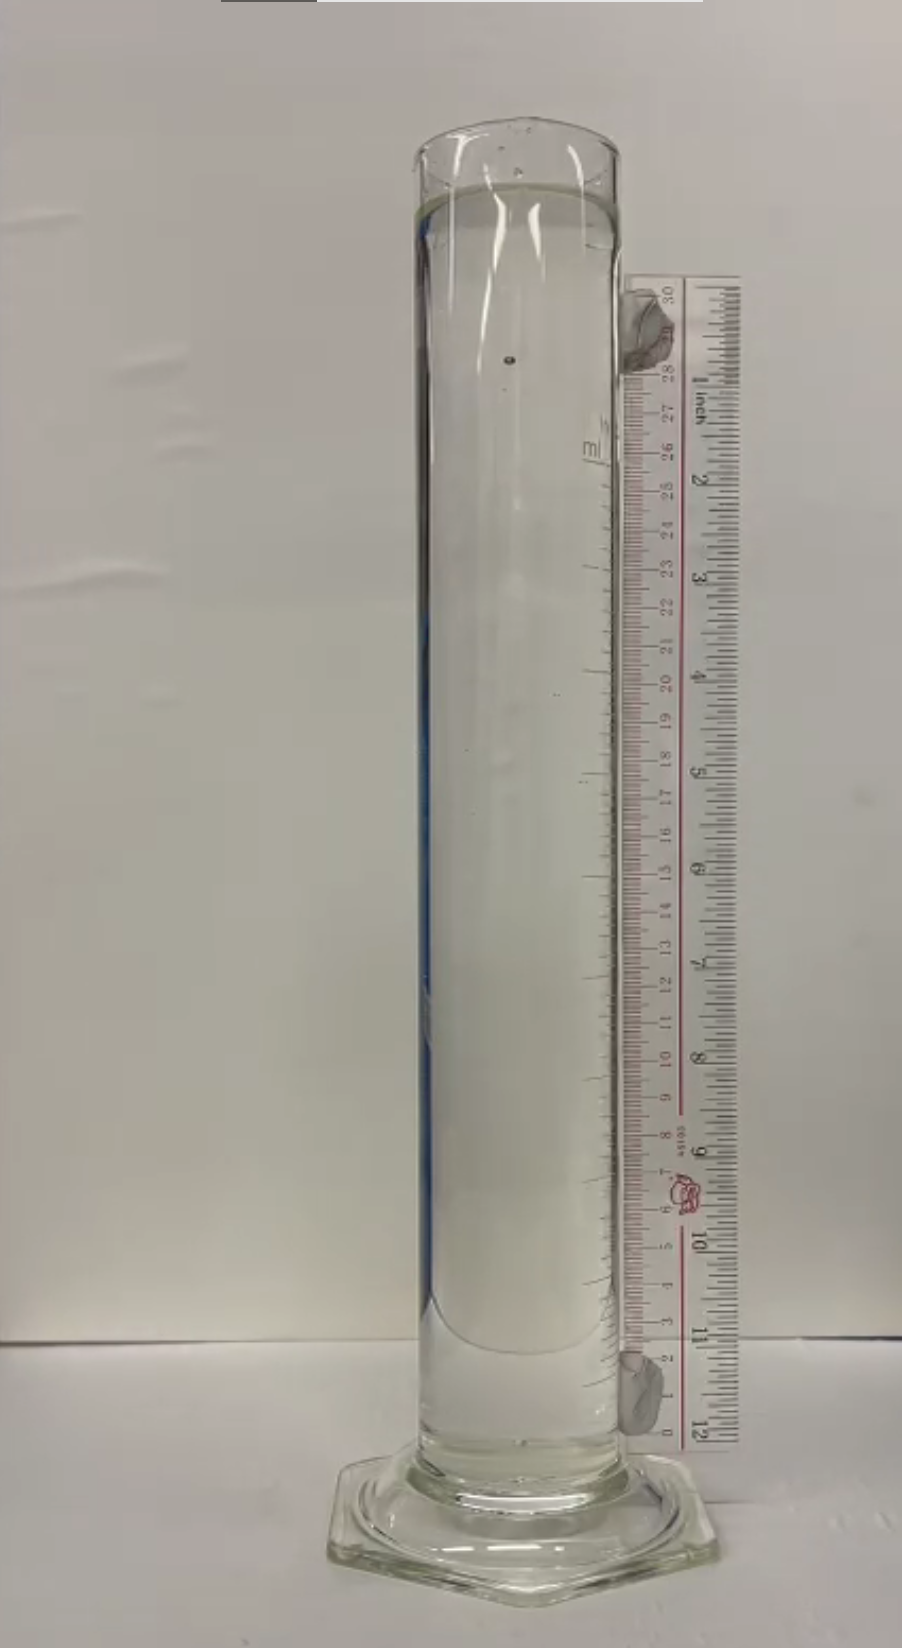
\includegraphics[height = 6cm]{Auxiliary Files/ENGG1350 Experiment Data/1350 image_1.png}
}
\subfigure[Large Particle]{
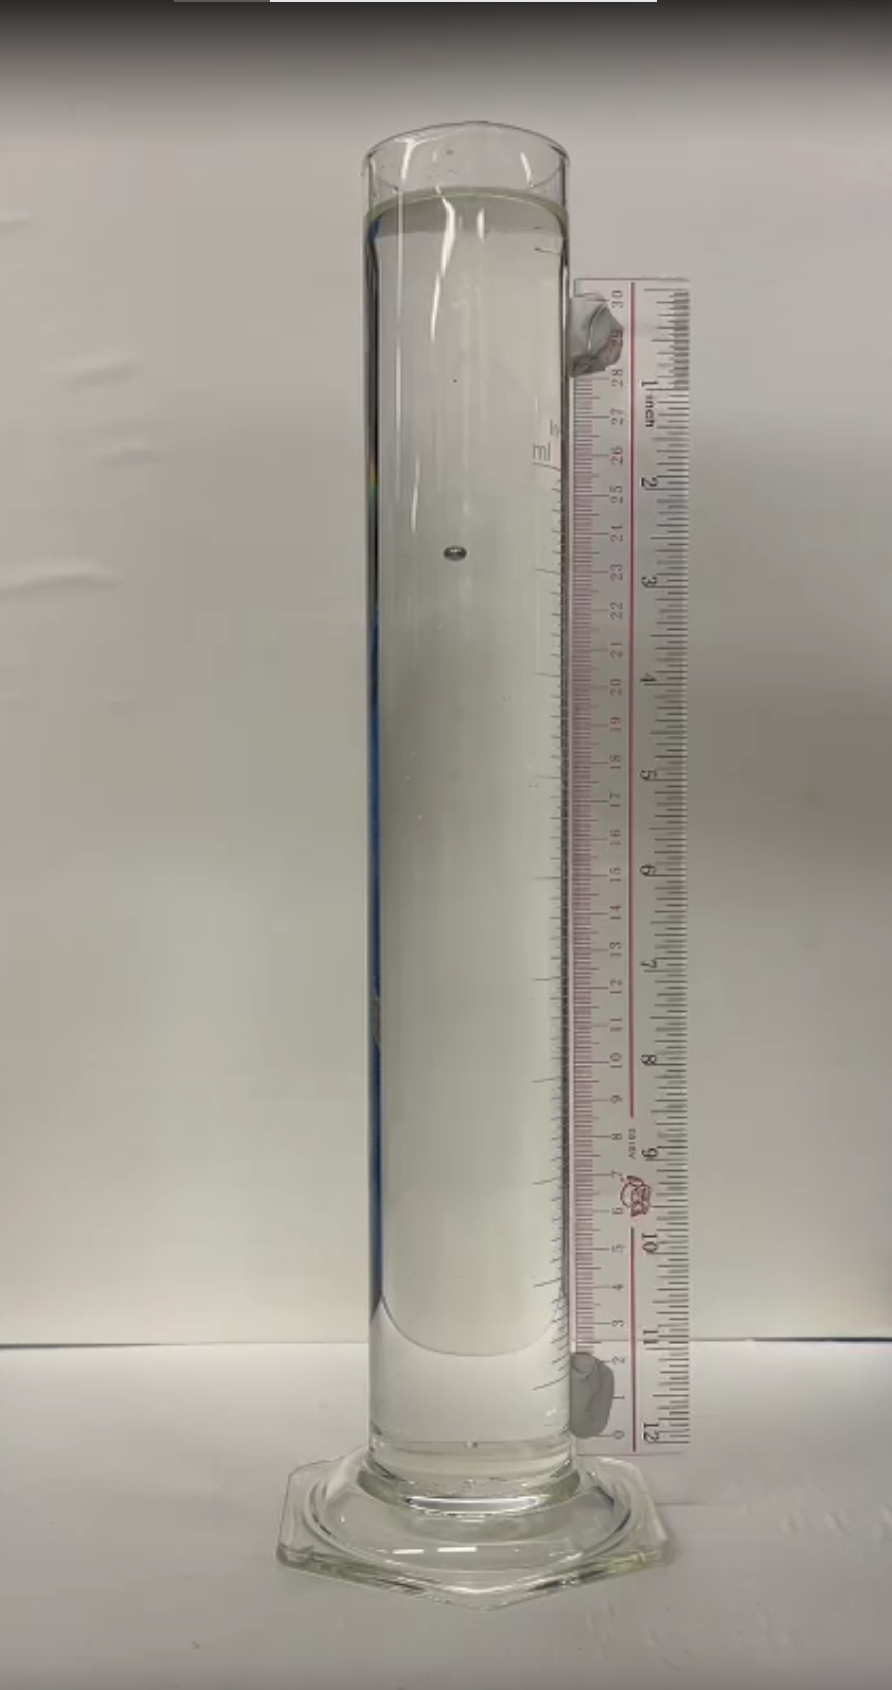
\includegraphics[height = 6cm]{Auxiliary Files/ENGG1350 Experiment Data/1350 image_2.png}
}
\subfigure[Tracker Software]{
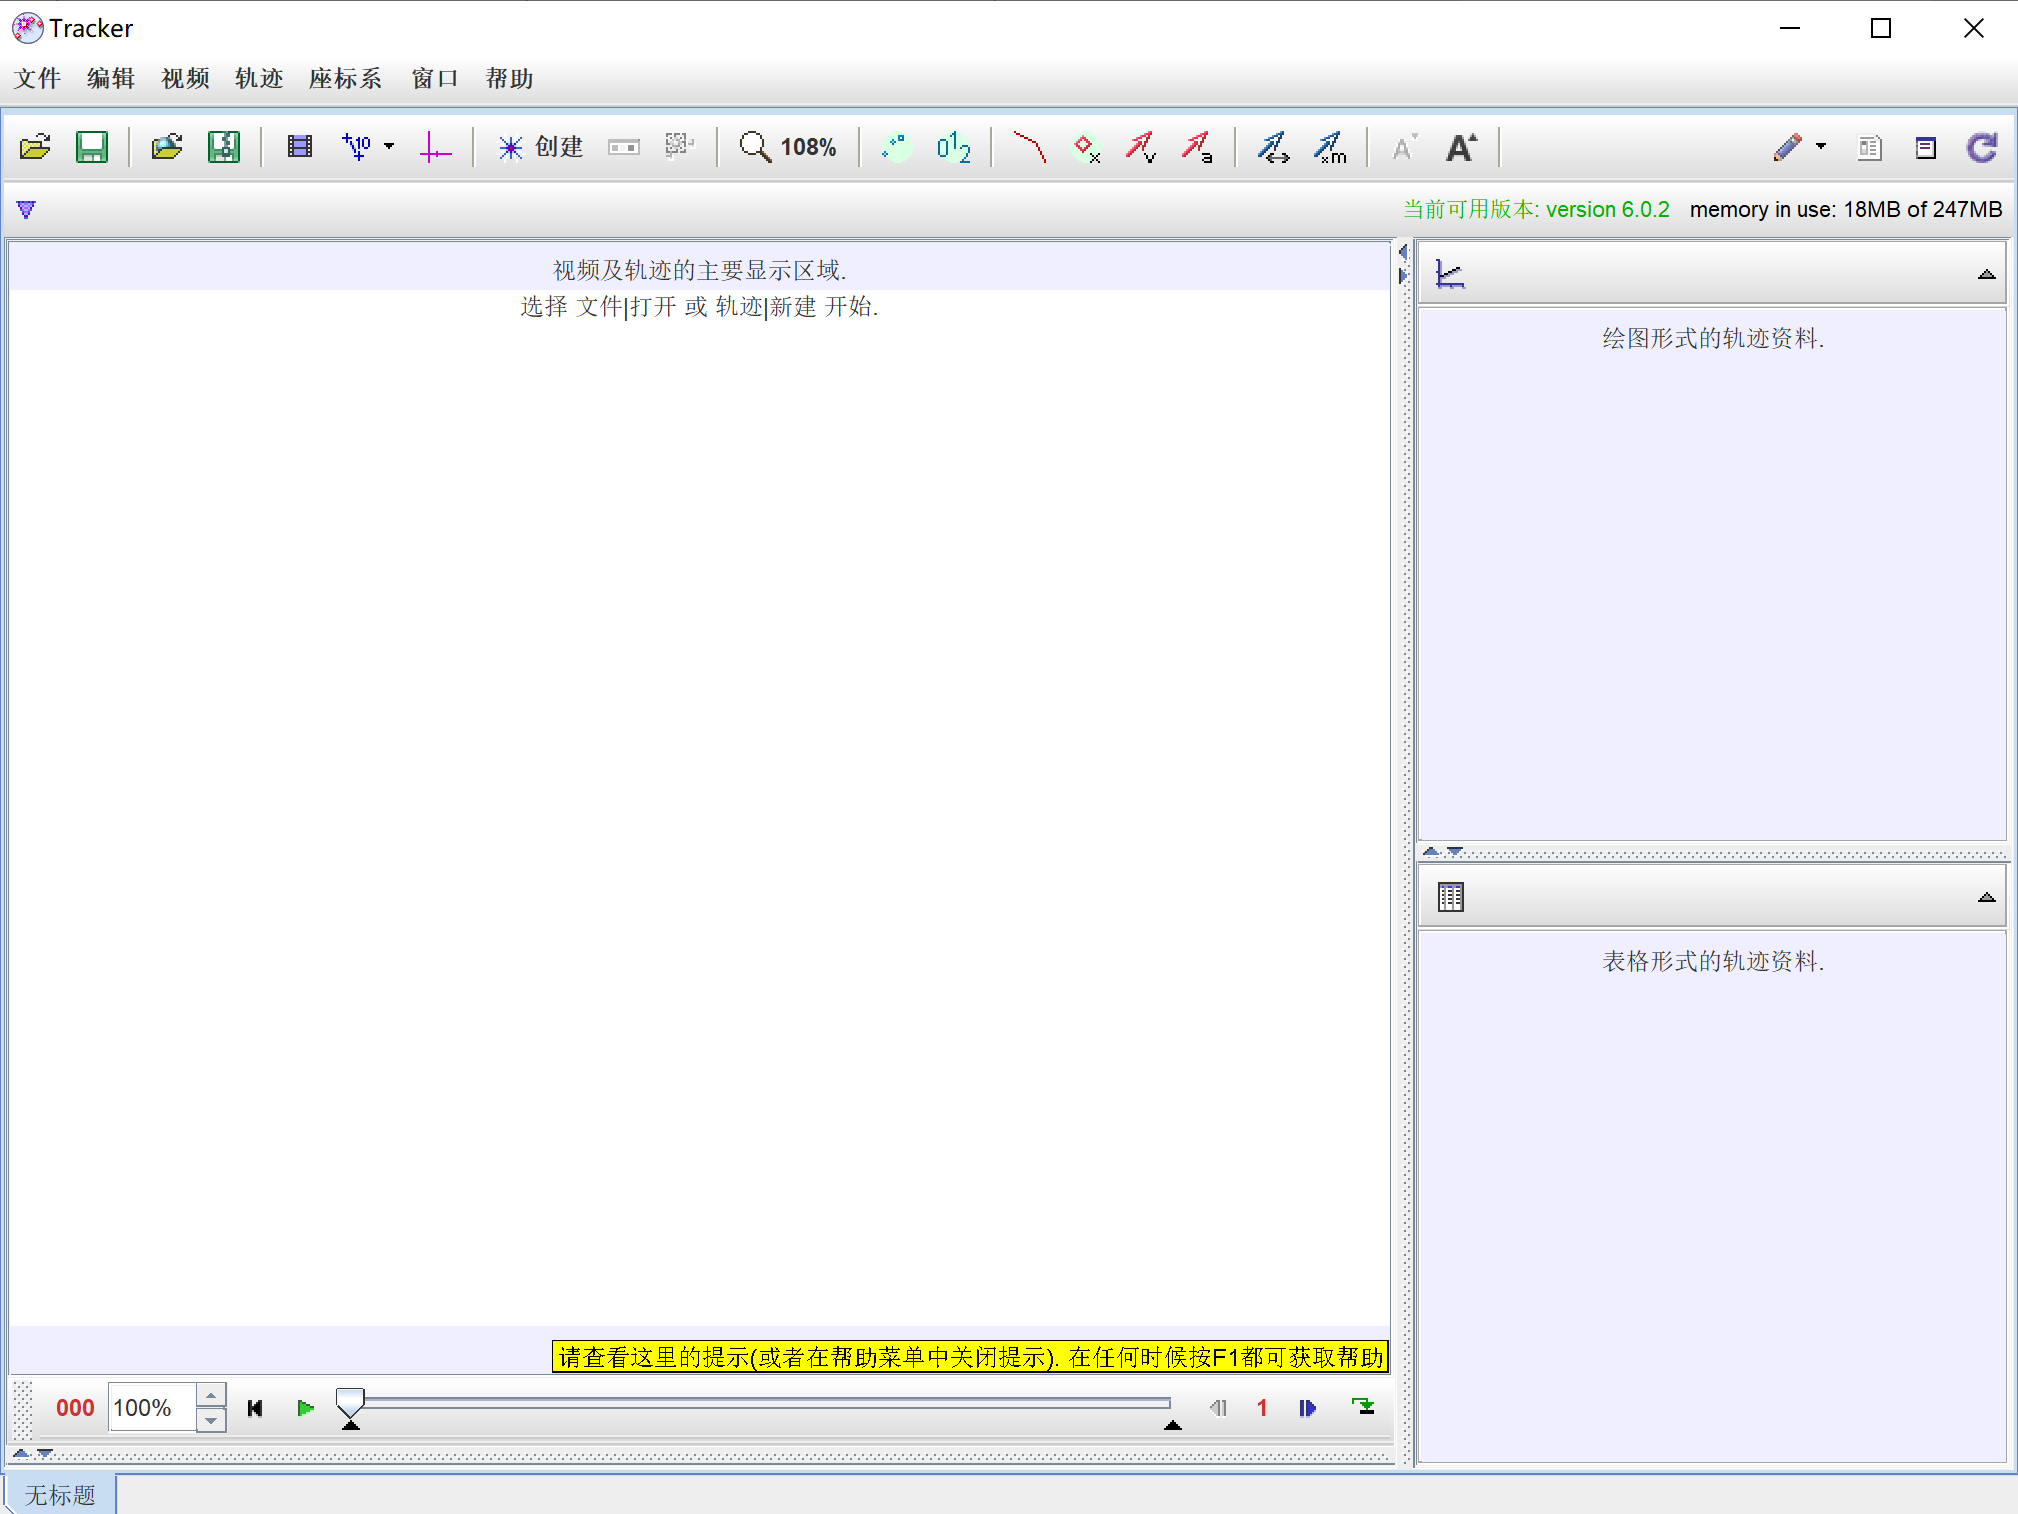
\includegraphics[height = 6cm]{Auxiliary Files/ENGG1350 Experiment Data/Tracker.png}
}
\end{figure}
\clearpage
\subsection{Result and Analysis}
\subsubsection{Data before Experiment}
\indent
\begin{table}[H]
\centerline{
\begin{tabular}{@{}lll@{}}
\toprule
Smaller particle & $D_1 = 1.98 \times 10^{-3} m /s$ & $M_1 = 0.033 \times 10^{-3} kg$ \\ \midrule
Larger particle  & $D_2 = 3.90 \times 10^{-3} m/s$ & $M_2 = 0.263 \times 10^{-3} kg$ \\ \bottomrule
\end{tabular}
}
\caption{Diameter \& Mass}
\label{tab:my-table}
\end{table}
\indent
\begin{table}[H]
\centerline{
\begin{tabular}{@{}ll@{}}
\toprule
Smaller particle & $\rho_{s_{1}} = \frac{6M_1}{\pi D_1^3} = 8119.321 kg / m^3$ \\ \midrule
Larger particle  & $\rho_{s_{2}} = \frac{6M_2}{\pi D_2^3} = 8467.658 kg / m^3$ \\ \bottomrule
\end{tabular}
}
\caption{Density}
\label{}
\end{table}
\indent
\subsubsection{Data in Experiment}
\indent
\begin{table}[H]
\centering
\begin{tabular}{|l|l|l|l|l|}
\hline
\multirow{3}{*}{Particle} & \multicolumn{3}{l|}{Terminal Velocity ($m/s$)}                                                      & \multirow{3}{*}{Average terminal velocity $\bar V$ ($m/s$)} \\ \cline{2-4}
                          & \multirow{2}{*}{First trail} & \multirow{2}{*}{Second trial} & \multirow{2}{*}{Third trial} &                                            \\
                          &                              &                               &                              &                                            \\ \hline
\multirow{2}{*}{Large}        & \multirow{2}{*}{0.06082}     & \multirow{2}{*}{0.06068}      & \multirow{2}{*}{0.06077}     & \multirow{2}{*}{0.06076}                   \\
                          &                              &                               &                              &                                            \\ \hline
\multirow{2}{*}{Small}        & \multirow{2}{*}{0.01682}     & \multirow{2}{*}{0.01677}      & \multirow{2}{*}{0.01679}     & \multirow{2}{*}{0.01679}                   \\
                          &                              &                               &                              &                                            \\ \hline
\end{tabular}
\caption{Velocity}
\label{tab:my-table}
\end{table}
\indent
\begin{table}[H]
\centering
\begin{tabular}{|l|l|l|}
\hline
\multirow{3}{*}{Particle} & Dynamic viscosity       & Reynolds number          \\
                          & \multirow{2}{*}{$\mu = \frac{(\rho_s - \rho_f)gD^2}{18 \bar V}$}      & \multirow{2}{*}{$Re = \frac{\rho_f D \bar V}{\mu}$}       \\
                          &                         &                          \\ \hline
\multirow{2}{*}{Large}    & \multirow{2}{*}{0.9840} & \multirow{2}{*}{0.3005}  \\
                          &                         &                          \\ \hline
\multirow{2}{*}{Small}    & \multirow{2}{*}{0.8734} & \multirow{2}{*}{0.04751} \\
                          &                         &                          \\ \hline
\end{tabular}
\caption{Outcome}
\label{tab:my-table}
\end{table}
\clearpage
\begin{figure}[H]
\centering
\subfigure[Small Trial 1]{
  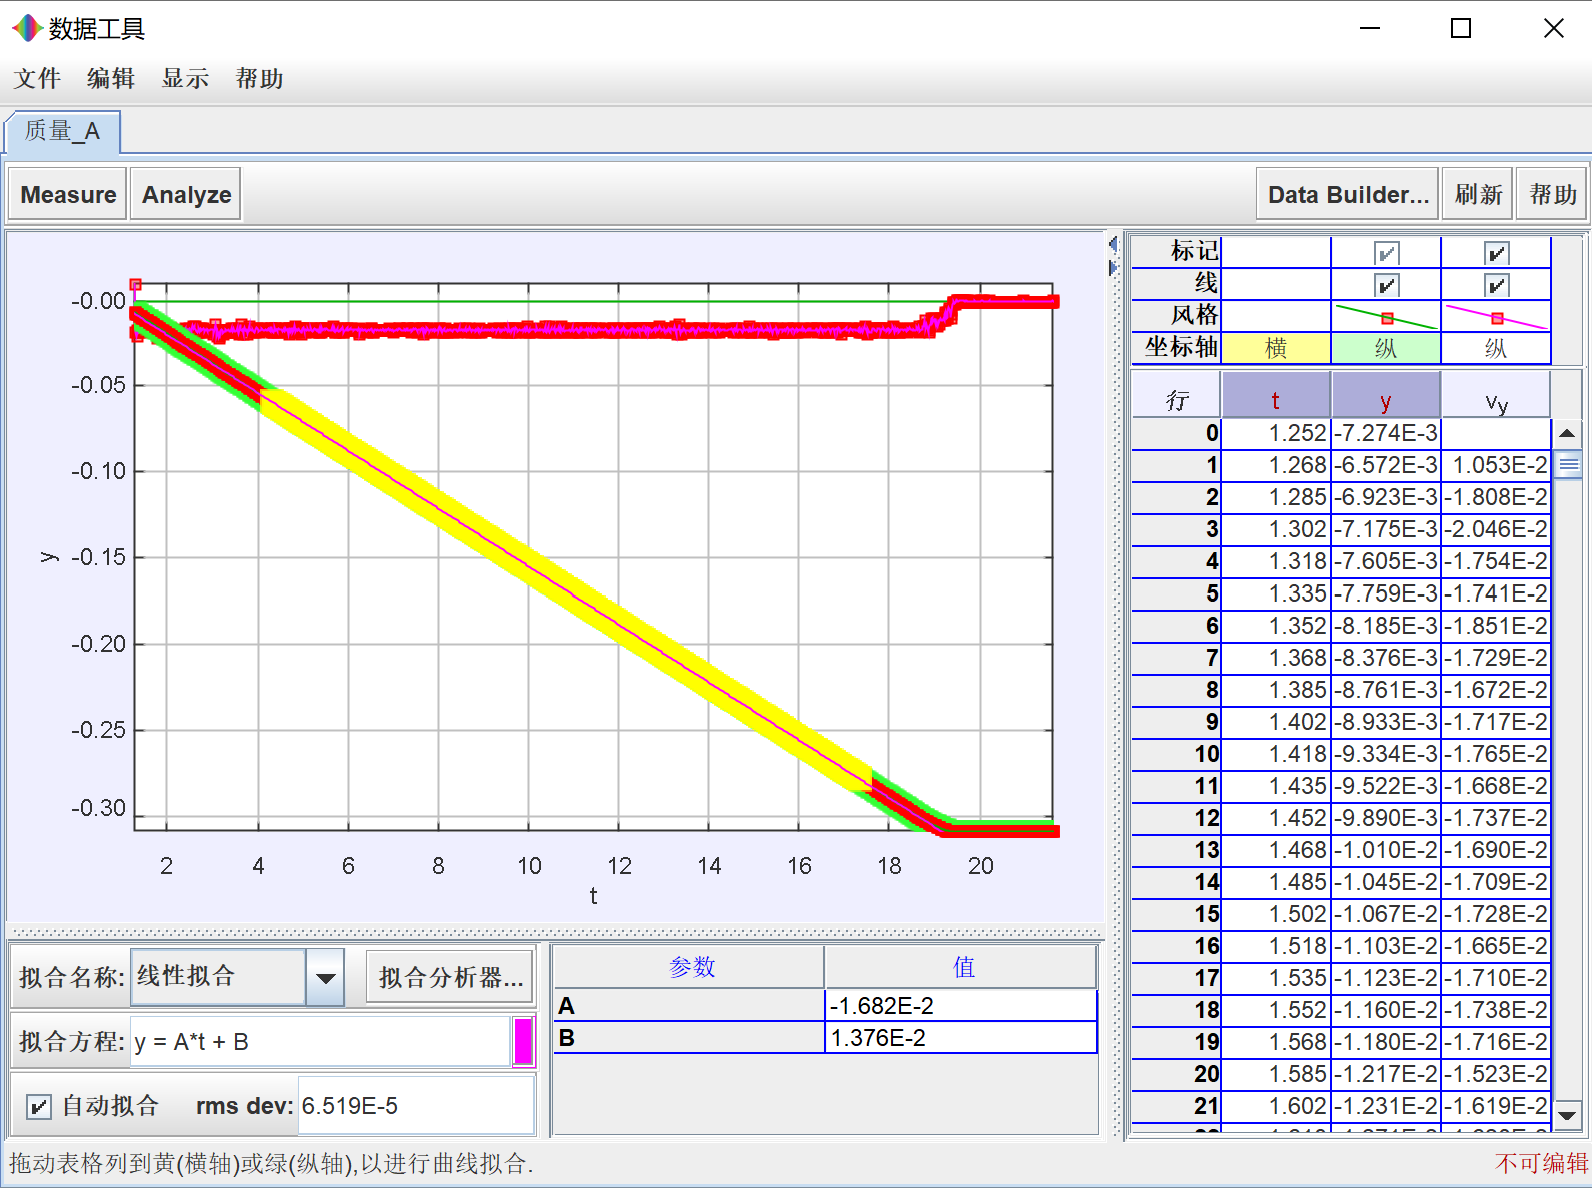
\includegraphics[width = 6.5cm]{Auxiliary Files/ENGG1350 Experiment Data/Data 1.png}
  \label{Trial_1}}
\quad
\subfigure[Small Trial 2]{
  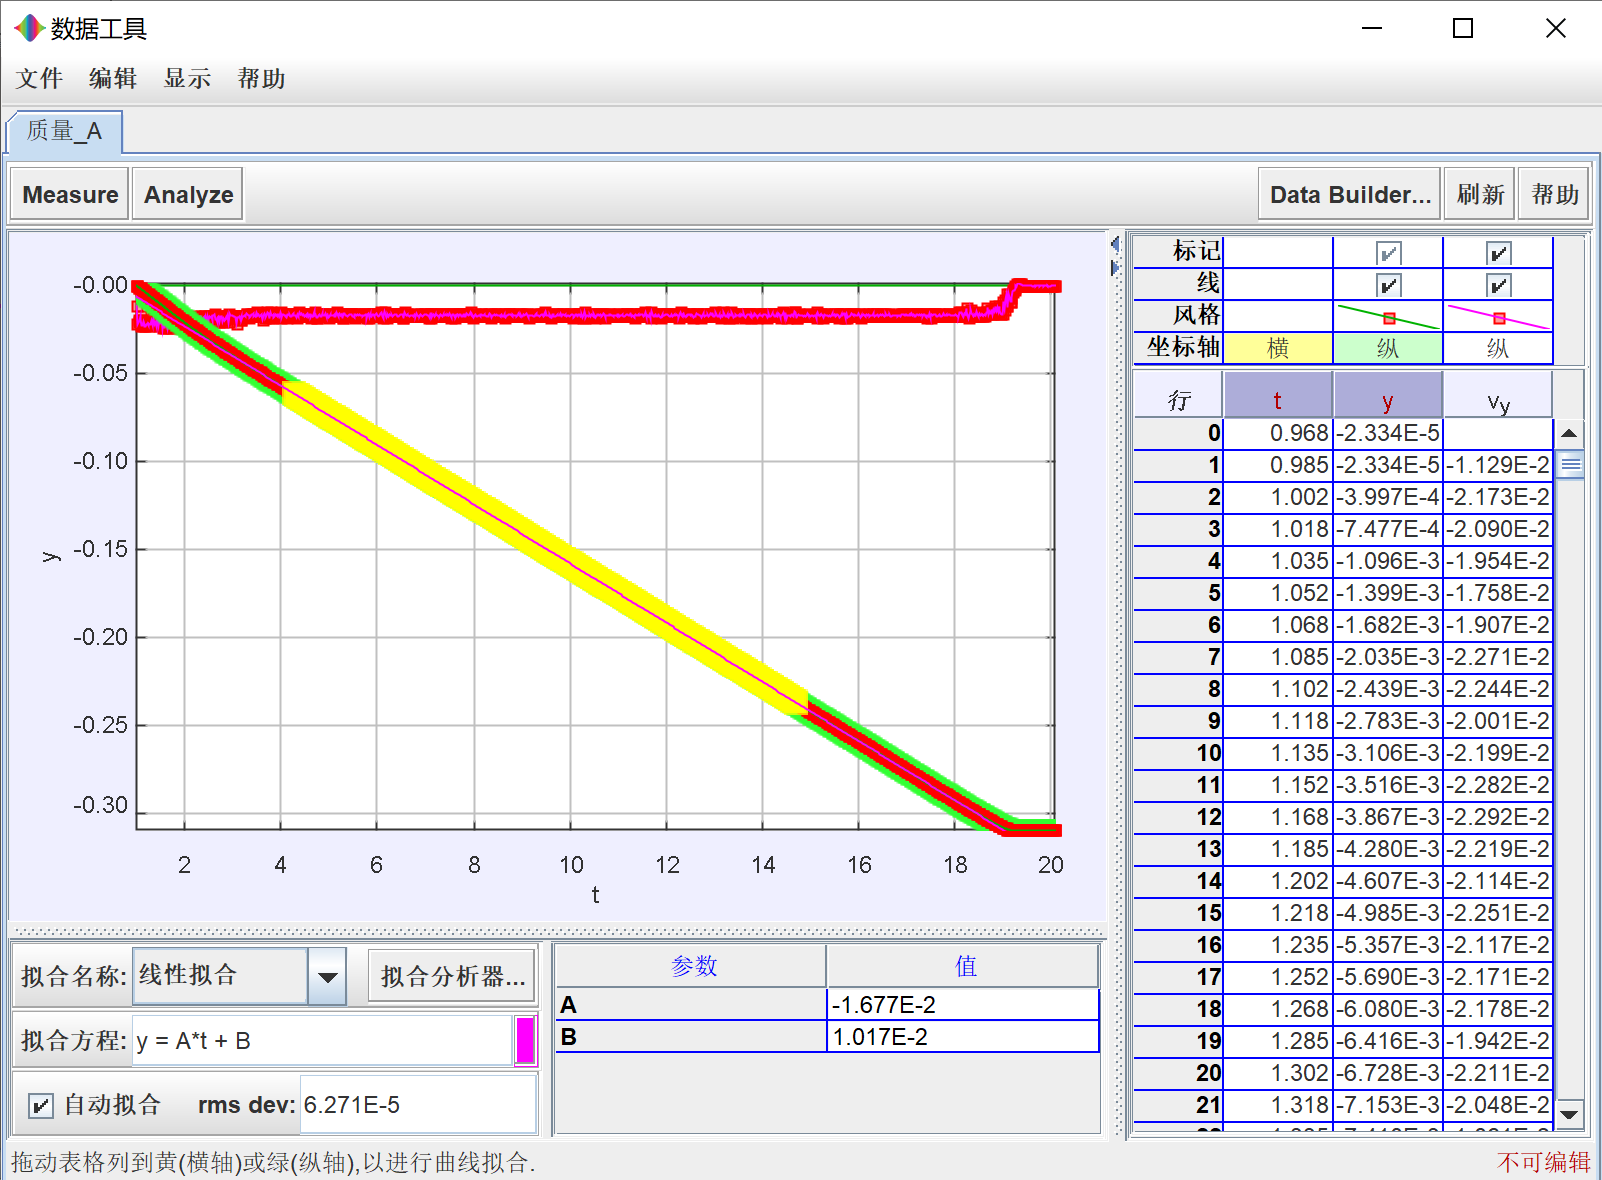
\includegraphics[width = 6.5cm]{Auxiliary Files/ENGG1350 Experiment Data/Data 2.png}
  \label{Trial_2}}
\subfigure[Small Trial 3]{
  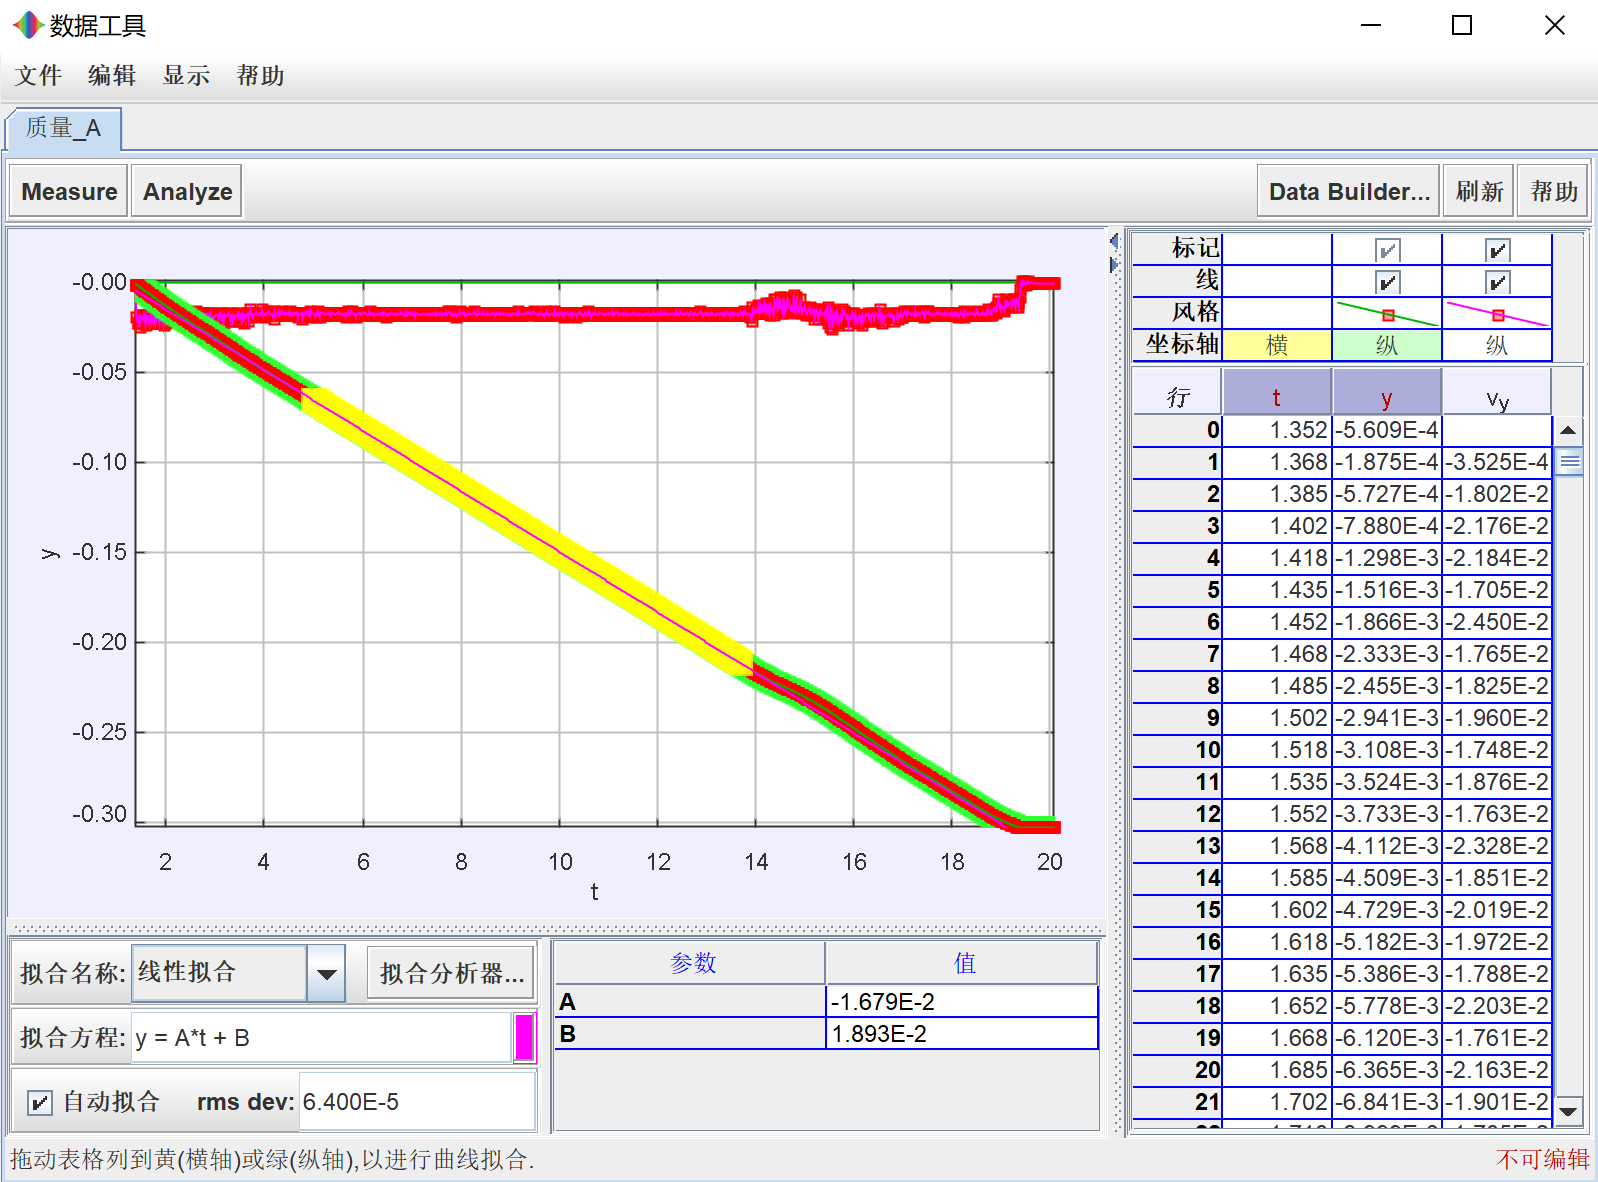
\includegraphics[width = 6.5cm]{Auxiliary Files/ENGG1350 Experiment Data/Data 3.png}
  \label{Trial_3}}
\end{figure}
\begin{figure}[H]
\centering
\subfigure[Large Trial 1 (Coordinate reversed)]{
  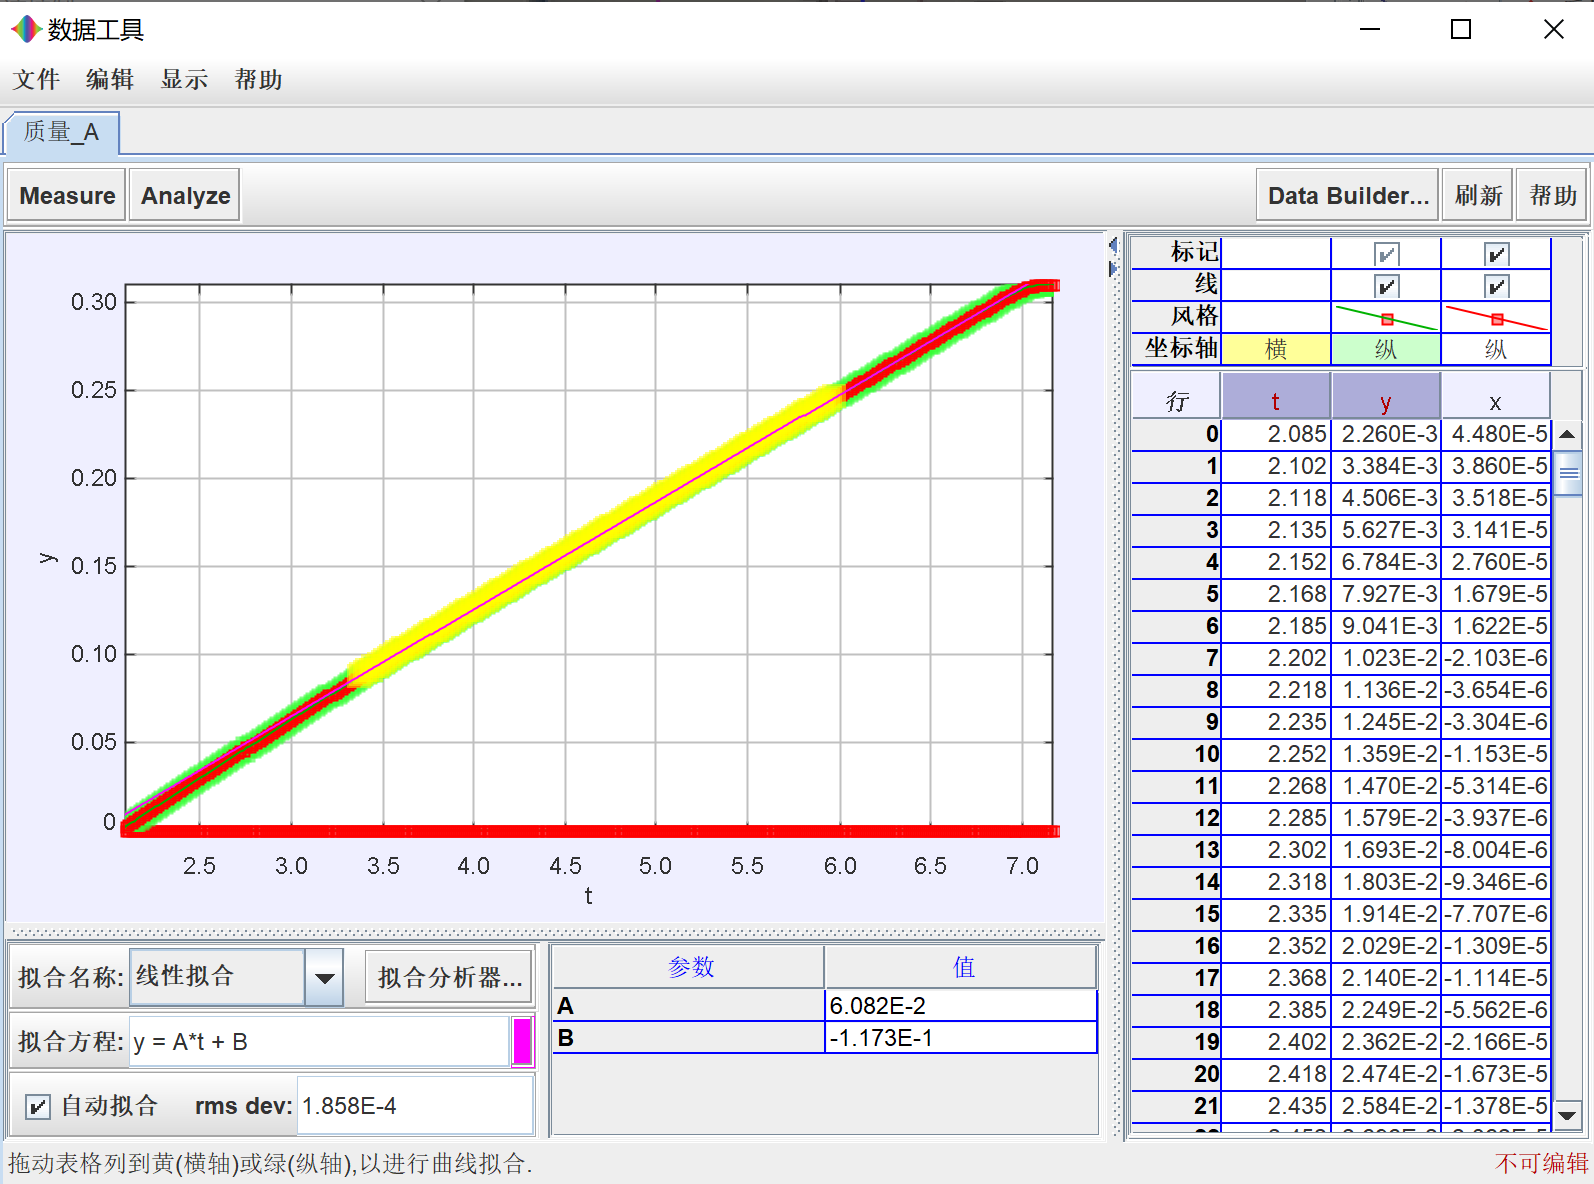
\includegraphics[width = 6.5cm]{Auxiliary Files/ENGG1350 Experiment Data/Data 4.png}
  \label{Trial_1}}
\quad
\subfigure[Large Trial 2 ]{
  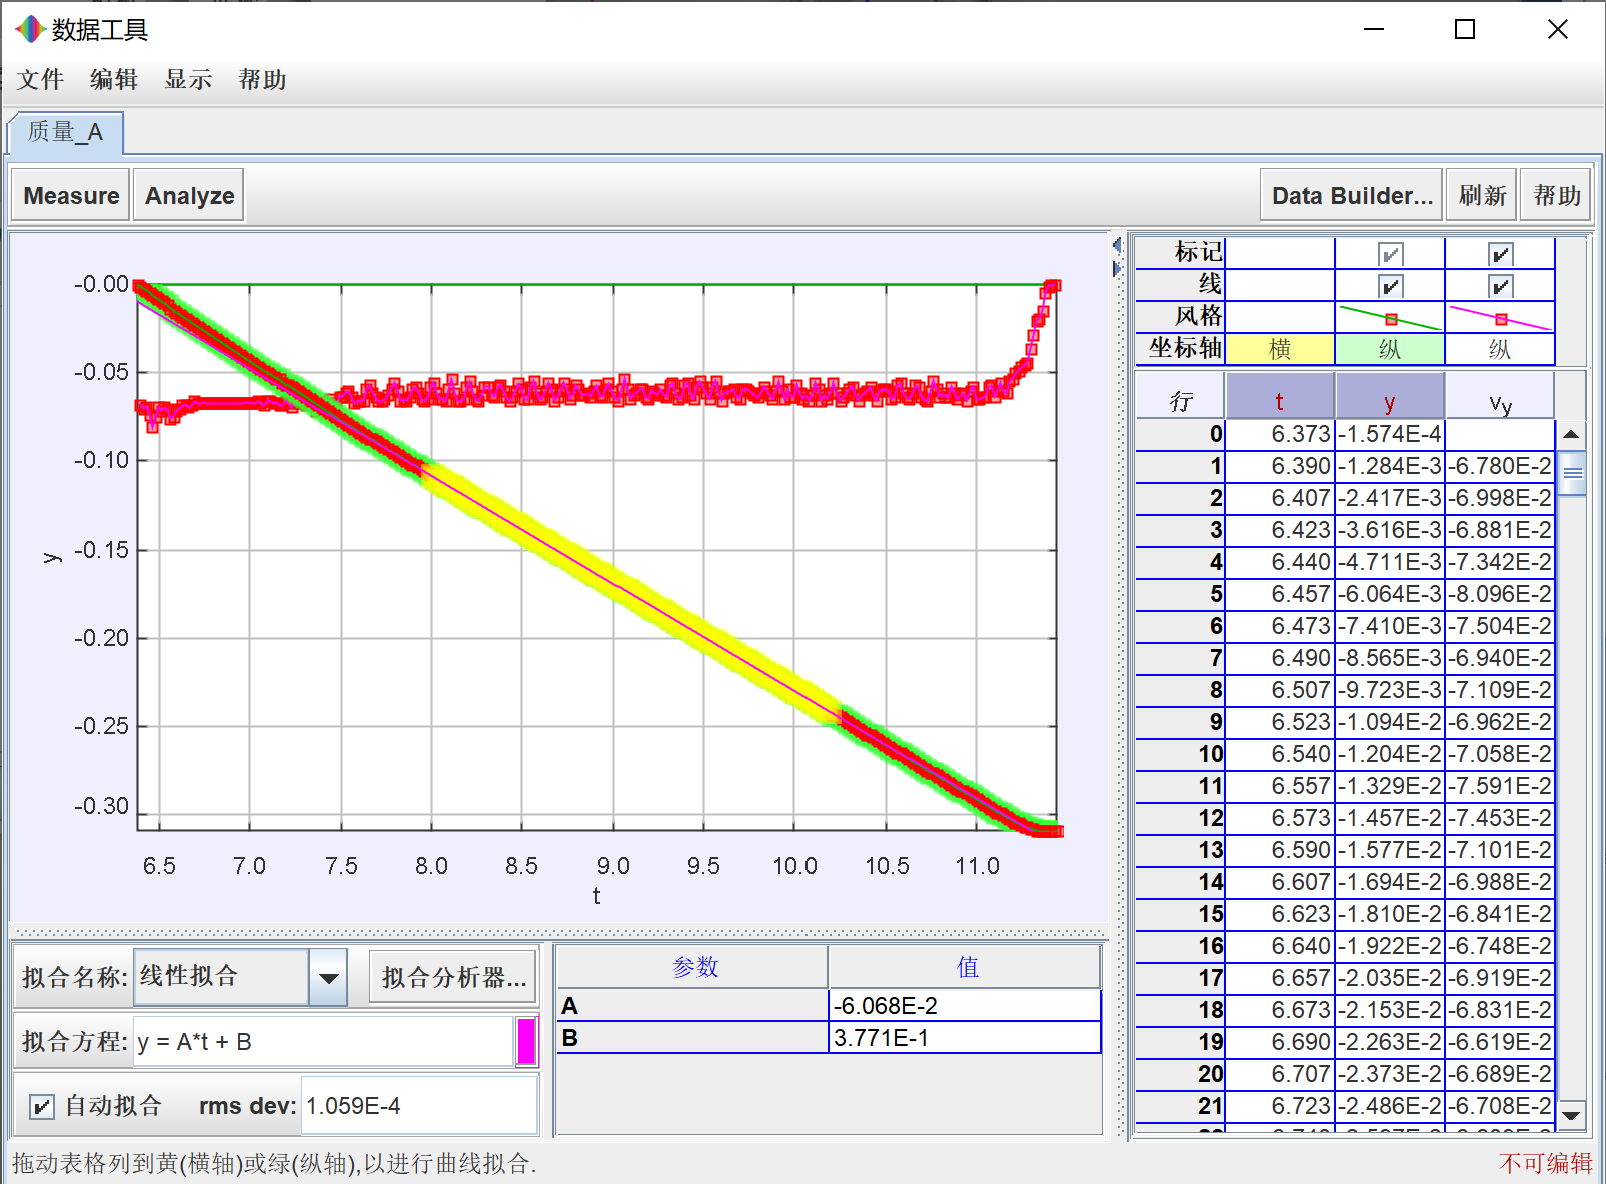
\includegraphics[width = 6.5cm]{Auxiliary Files/ENGG1350 Experiment Data/Data 5.png}
  \label{Trial_2}}
\subfigure[Large Trial 3 (Coordinate reversed)]{
  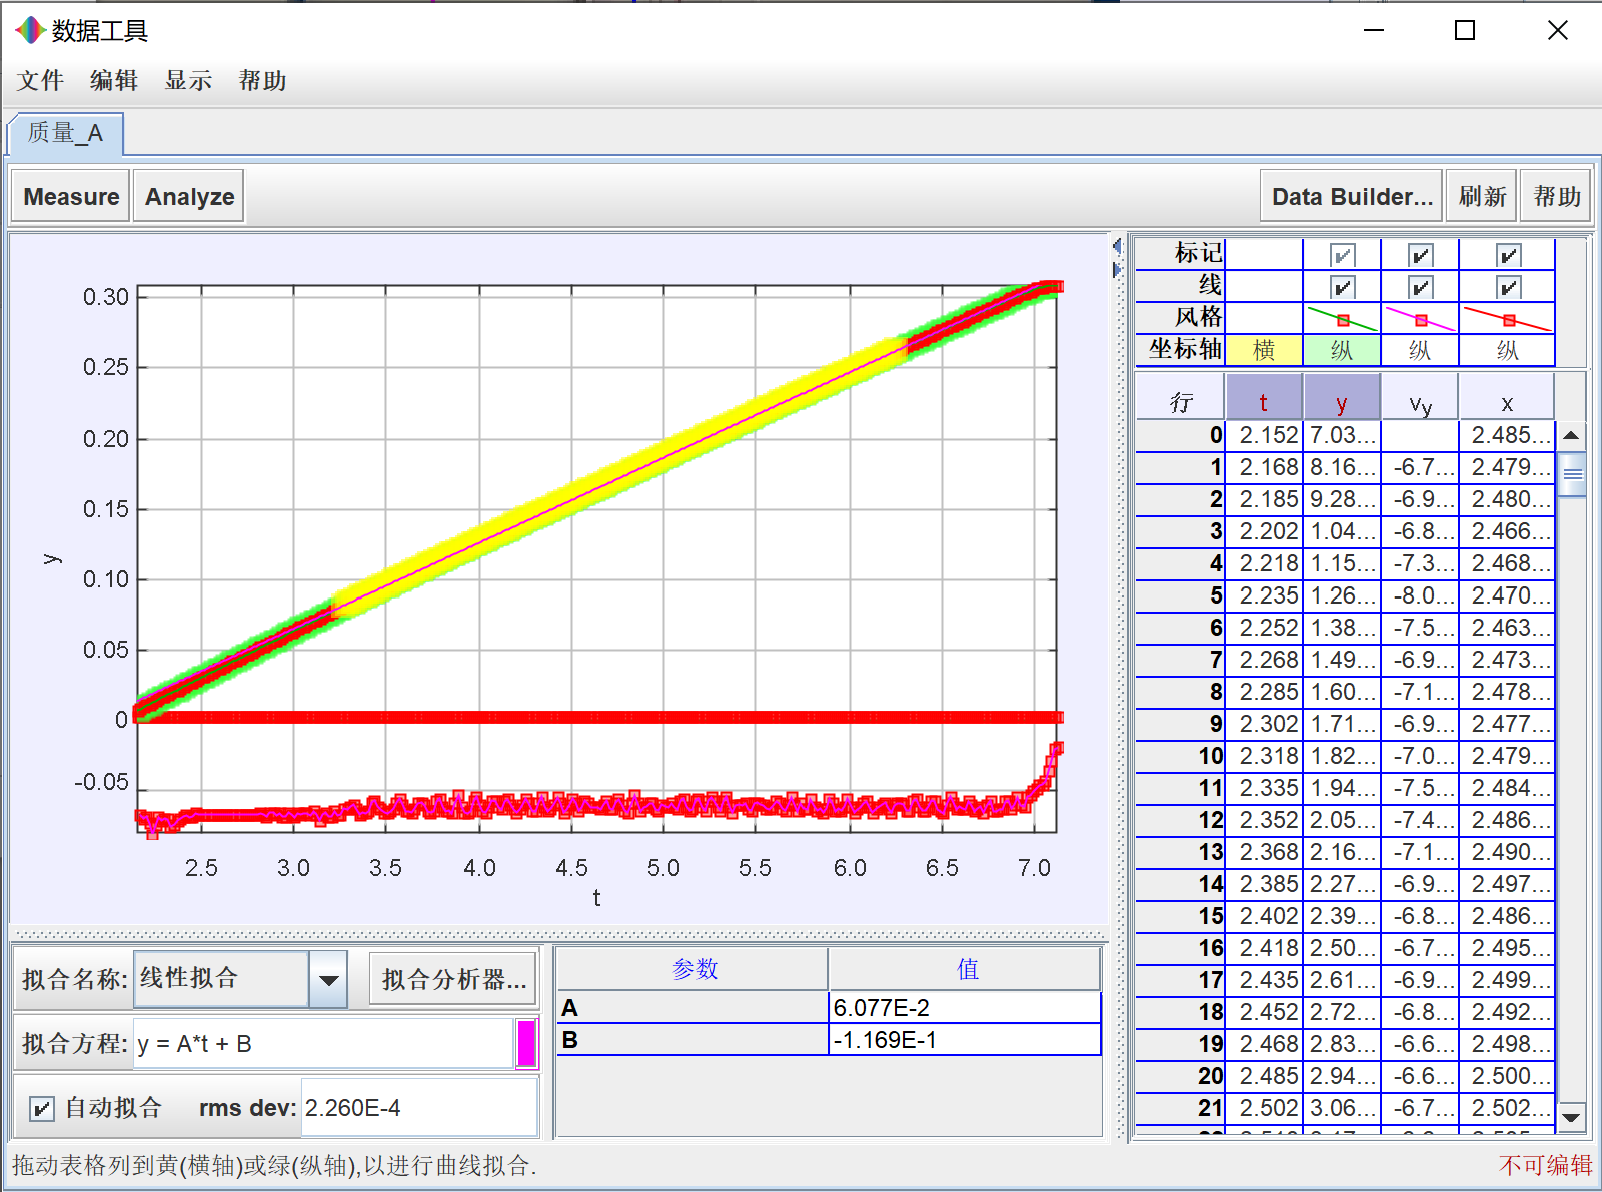
\includegraphics[width = 6.5cm]{Auxiliary Files/ENGG1350 Experiment Data/Data 6.png}
  \label{Trial_3}}
\end{figure}
\clearpage
\section{Analysis and Discussion}
\textcircled{\small 1} To analyse the two measured values, we define \textbf{\textit{relative difference}} as
\begin{equation}
\begin{aligned}
    \eta &= \frac{|\mu_1 - \mu_2|}{\frac{\mu_1 + \mu_2}{2}} \\
    & = 0.119
\end{aligned}
\end{equation}
The two measured values are slightly different.The difference may be caused by \textbf{insufficiency of instrumental accuracy, error of experiment operation, inaccuracy of object tracking in \textit{Tracker} software, some turbulence occurred in the falling process, etc.}
\par
\textcircled{\small 2} For the small particle the prerequisite that $Re << 1$ is satisfied. Nevertheless, for the large particle we can not obtain $Re << 1$. Thus the \textit{LHS} in equation ( 2 ) can not be simply neglected. The existence of extra viscosity brought by Reynolds number provides the particle with an extra drag force, which contributes to the error of the measured value in this experiment.
\par
\textcircled{\small 3} According to the table of dynamic viscosity \footnote{https://www.engineeringtoolbox.com/absolute-viscosity-liquids-d1259.html}, the density and average dynamic viscosity of the fluid we measured in this experiment best corresponds \textbf{Glycerine}.
\begin{figure}[H]
    \centering
    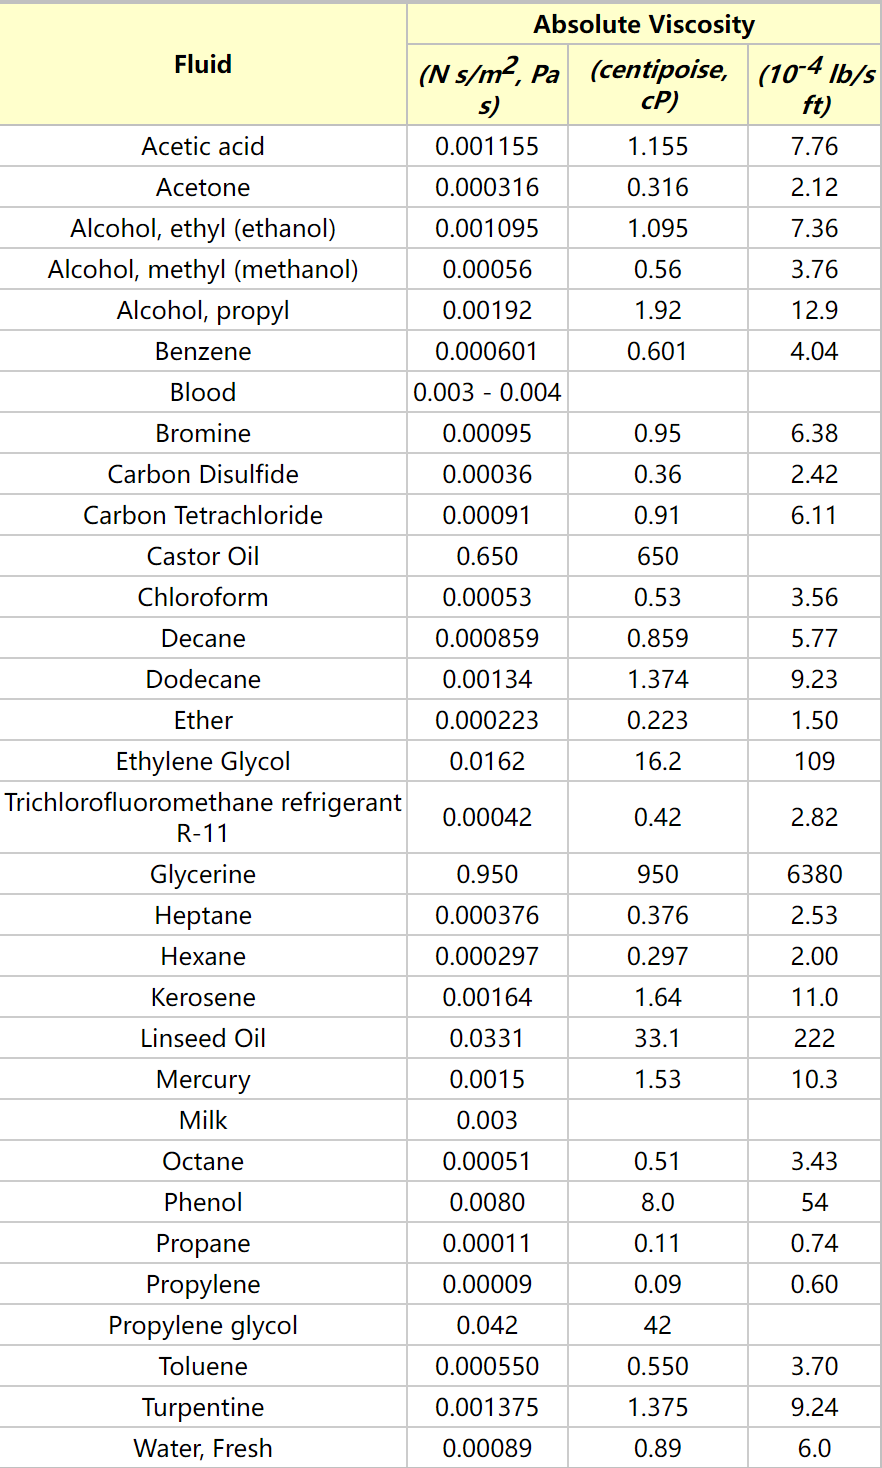
\includegraphics[height = 14cm]{Auxiliary Files/ENGG1350 Experiment Data/Dynamic Viscosity.png}
    \caption{Fluid Feature Table}
    \label{fig:my_label}
\end{figure}
\clearpage
\section*{References}
[ 1 ] Nptelhrd. (2015, June 22). Mod-01 Lec-18 Stokes Drag on a Sphere (Contd.) and Introduction $~~~~~~~~~~~~~$to Lubrication Theory. Youtube. https://www.youtube.com/watch?v=v8juW2d2tYc\&t=989s
\par
\indent
\par
\indent [ 2 ] Nptelhrd. (2015, June 22). Mod-01 Lec-17 Stokes Drag on a Sphere. Youtube. \par \noindent $~~~~~~~~~~~~$https://www.youtube.com/watch?v=v8juW2d2tYc\&t=989s
\par \indent \par 
\indent [ 3 ]吴耀祖. (1981). 低雷诺数流体力学介绍. 力学与实践, 34–40+54. 
\end{document}